% !TEX root = main.tex

\chapter{Experimental results}
This chapter collects all the experimental results obtained during the thesis. Apart from the AOD characterization, there are two main sections. The first one contains the measurements carried out on the test setup done to asses the performance of the system. Here, polarization, stability, and focus spot has been checked. In particular, two methods have been used to measure $\mu$m focus spot: razor blade scans, and small pixel size camera. The other section comprises more advanced quantum optic experiments realized with ions and the final installed system. Ramsey spectroscopy was used to check addressing error and focus spot. Moreover, photons have been generated from one single ion with adjacent unperturbed ions.

\section{AOD}
The AOD is the core element of the setup, it is therefore essential to characterize it. The two main parameters we are interested in are the diffraction efficiency and the response time. For the diffraction efficiency we measure the total output power of the light $P_{tot}$ and then the power of the first diffracted order $P_{1}$. Diffraction efficiency is defined as the ratio between the two.
\begin{equation}
\text{DE} = \frac{P_1}{P_{tot}}.
\end{equation}
Before measuring the diffraction, the optimal RF power to drive the AOD has been found. This was done by measuring the power at the central frequency of the AOD and maximizing the light in the first diffracted order. Power measurements of the light were done with a Thorlabs PM100D, and the AOD was driven with a signal generator. The optimal RF power was found to be 0.11 W, and for the rest of the measurements it was kept as that value. Furthermore, the input polarization was optimized with a half wave plate, always trying to maximize the power of the diffracted light. In figure \ref{DE} the plot of the diffraction efficiency as a function of the RF frequency is displayed. Within a bandwidth of 50 MHz from 105 MHz to 155 MHz, we can see that more than 70 \% of the light is in the first diffracted order as expected from the datasheet, even though the bandwidth looks shifted with respected to the nominal central frequency of 120 MHz.\\
The response time is the time that it takes for the light to move when the RF frequency is changed. In order to perform this measurement, a voltage controlled oscillator (VCO) was used to generate the RF signal. The VCO was supplied a square wave that jumped between two voltages corresponding to two different frequencies. The blue light was measured with a photodiode. The photodiode was aligned with the light at one particular frequency, such that when the light moves, the beam would not hit the chip and the signal generated changes. In figure \ref{response}, the signal of the photodiode, together with the supplied VCO signal are plotted. Response time is $\sim 7-8\,\mu$s, in this time the light completely move from one angle to another one.

\begin{figure}
\centering
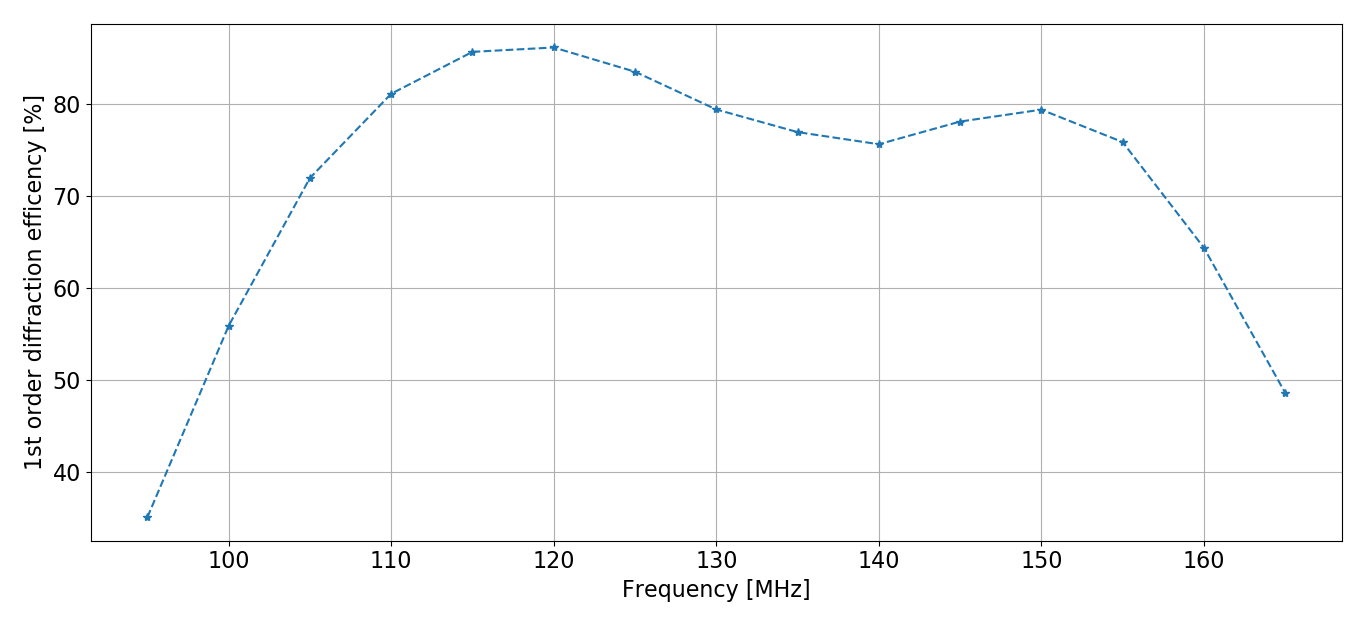
\includegraphics[width = .95\textwidth]{DE}
\caption{Diffraction efficiency of the AOD as a function of the RF driving frequency.}
\label{DE}
\end{figure}

\begin{figure}
\centering
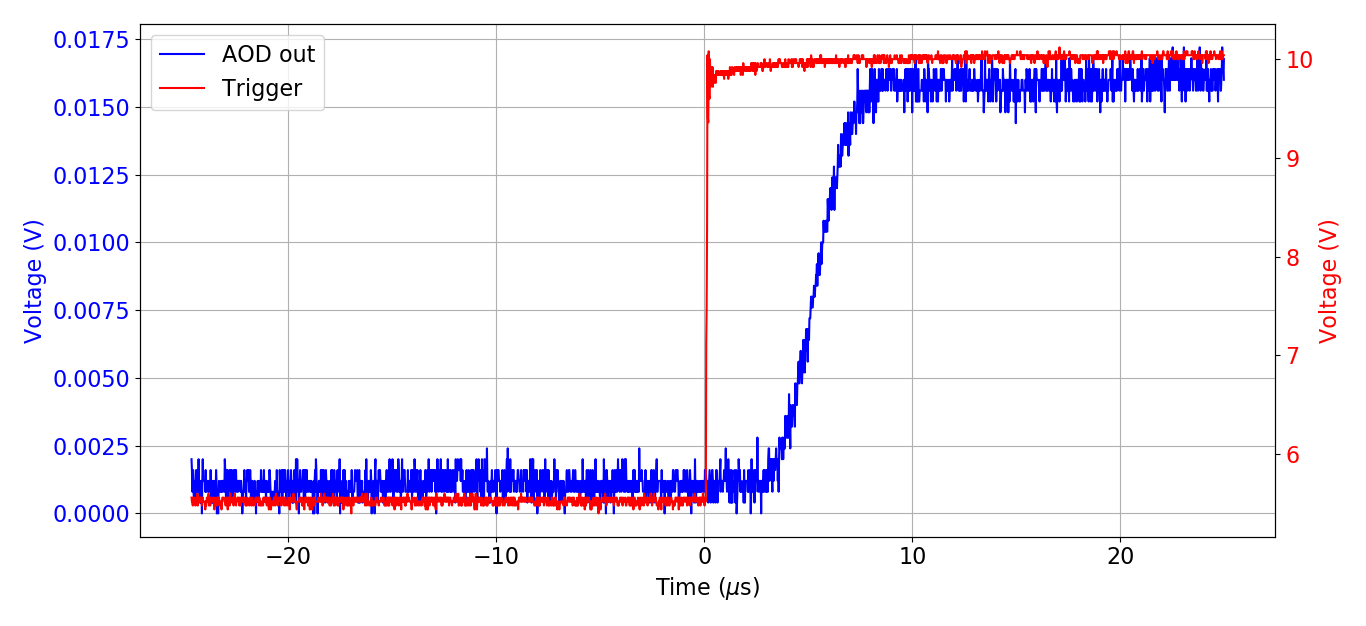
\includegraphics[width = .95\textwidth]{response}
\caption{Response time of the AOD, plotted are the photodiode signal in blue on the left $y$ axis, and the VCO voltage is in red on the right axis.}
\label{response}
\end{figure}

\section{Full test setup characterization}
The test setup was built on a spare optical table with a spare objective. The layout of the setup was as close as possible to the final version, so the system in figure \ref{addressingsetup} was replicated. The most important assessment was the focus spot, i.e. we tried to measure the waist of the beam and check if it was within requirements.
This is measured in two different ways: first we used a technique called Knife-edge, where the beam is scanned with a razor blade; then we also tried to measure it directly with a camera equipped with 1.6 $\mu$m pixel size.\\
Other than the waist size, we also measured stability of the system and the polarization capabilities.

\subsection{Waist: Knife-Edge method}
\begin{figure}[H]
\centering
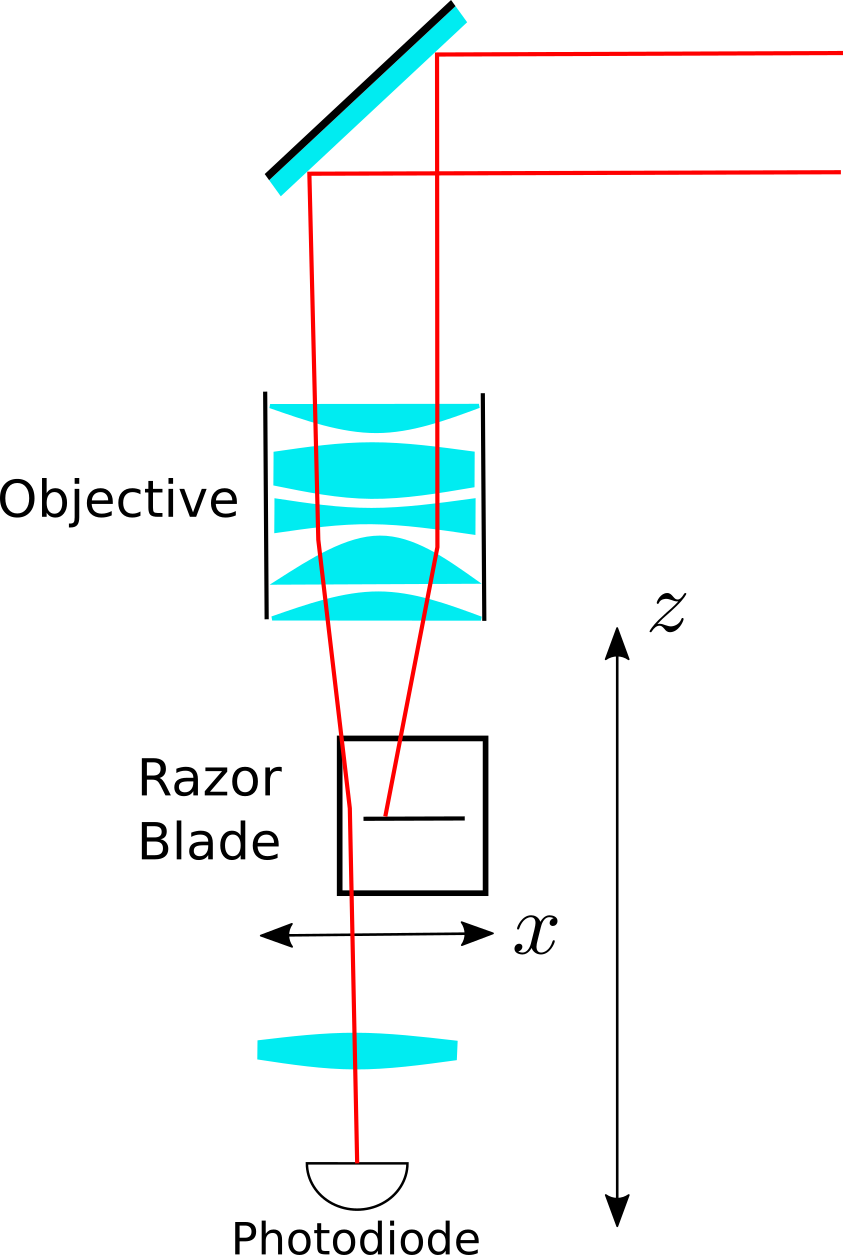
\includegraphics[scale = 1.1]{razorsetup}
\caption{Scheme of the razor scan.}
\label{razorscan}
\end{figure}
Measuring a micrometer waist is not easy task, the first approach we tried consists of mounting a razor blade on a translational stage. The stage is then moved in the $x$ direction cutting the beam perpendicularly such that the blade is scanning the beam profile. The setup used is showed in figure \ref{razorscan}, after the objective the blade is present, and since the beam is quickly diverging after the focus, a lens is used to refocus the light into a photodiode. A filter was also inserted in order to not saturate the photodiode.
In the $z$ direction the stage was controlled with a manual screw with resolution of $1\,\mu$m. While in the $x$ direction, the stage had to be moved with sub-micrometer precision, so the screw was a piezo actuator controlled by custom software. The same software also controlled a multimeter that measured the voltage of the photodiode. To get the whole profile of the beam, i.e. $W(z)$, the measurement procedure was as follow
\begin{itemize}
\item Position blade at appropriate $z$ coordinate
\item Scanning beam in $x$ direction with blade
\item Beam width extrapolation
\item Shift $z$ direction
\end{itemize}
And the procedure is repeated for sufficient values of $z$ to scan at least few Raylegh ranges. The beam width can be calculated from the scans by fitting the data with \cite{knifeedge}
\begin{equation}
P(x,z) = \frac{P_0}{2}\text{erfc}\left[\frac{\sqrt{2}(x-x_0)}{W(z)} \right].
\end{equation}
Where the fitting parameters are $P_0, x_0,$ and the width $W(z)$. An example of scan is in figure \ref{examplerazorscan}. The errorbars comes from statistical average, every data point is a mean over 5 measurement, and the error is the standard deviation. The fit in this case gave a width of $3.47\pm 0.06\,\mu$m, the smallest width obtained with this method. Unfortunately, it is broader that the initial expectations. Furthermore, the profile $W(z)$ did not look symmetric and could not be fitted with equation \eqref{waistprofile}. A possible explanation is that this method is not suitable for measuring micrometer waists with a razor blade, the roughness of the surface could limit the result. In comparison, authors of \cite{Cannon:86} have used, instead of a common razor blade, a glass substrate etched with an effective knife-edge feature.
\begin{figure}
\centering
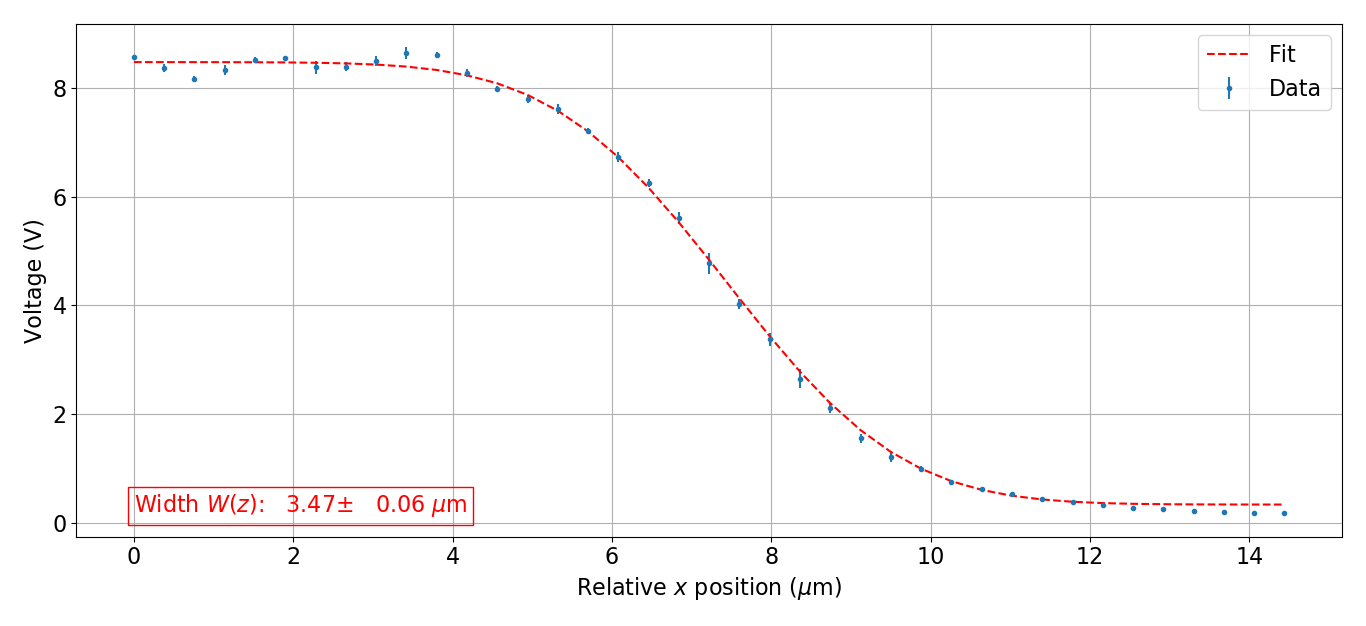
\includegraphics[width=1\textwidth]{img/razorscan}
\caption{Example of razor scan}
\label{examplerazorscan}
\end{figure}


\subsection{Waist: Camera}
\label{waistcamera}
Since the Knife-Edge method did not demonstrate particularly effective, if not to give an upper bound to the waist, a more direct approach has been subsequently adopted. We look directly into the beam with a camera from IDS model UI-1490LE-M-GL. This particular camera has a pixel size of 1.6 $\mu$m, with no pixel-pixel distance. It should therefore be suitable to measure a focus spot better than the razor blade. A $\mu$m focus should hit one single pixel, and if aligned between two pixels, a Gaussian profile could also be fitted.
In addition, unlike the Knife-Edge technique, a camera provides 2-dimensional information about the beam shape and can be exploited to look for aberrations in the system. The setup is almost the same as figure \ref{razorscan}, but the camera now replaces the razor blade, and there is no need for scanning in the $x$ direction, as the $z$ is enough to reconstruct the profile $W(z)$. An additional gradient filter was used to optimize the light reaching the camera in order to not saturate it and get a visible signal.
\begin{figure}
     \centering
     \begin{subfigure}[b]{0.67\textwidth}
         \centering
         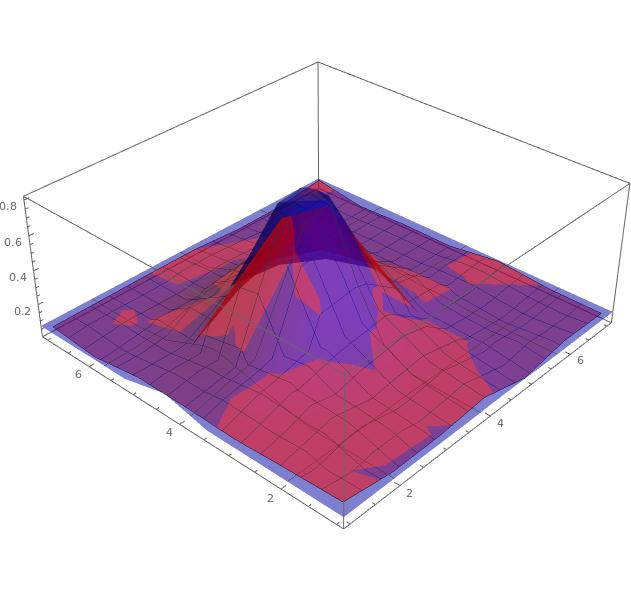
\includegraphics[width = \textwidth]{camera}
          \caption{Fitted data from the camera. In red color, the normalized pixel value is displayed, while the blue curve is a fitted 2D Gaussian. On the axis there is the pixel number}
     \end{subfigure}
     \hfill
     \begin{subfigure}[b]{0.3\textwidth}
         \centering
         
\includegraphics[width=\textwidth]{cameraoriginal}
        \vspace{5em}
         \caption{Original photo from the camera.}
         %\label{fig:three sin x}

     \end{subfigure}
        \caption{}
       \label{fig:camera}
\end{figure}
The measurement procedure is also similar to the Knife-Edge case. For every desired $z$ displacement, a photo with the camera is taken, post processed, and then the camera is displaced to the new $z$ coordinate. Post processing is done by fitting the pixel values with a 2-dimensional Gaussian
\begin{equation}
P = A \exp\left\{-\frac{(x-x_0)^2}{2\sigma_x^2}\right\} \exp\left\{-\frac{(y-y_0)^2}{2\sigma_y^2} \right\}.
\end{equation}
The fit parameters are $A,x_0,y_0,\sigma_x,$ and $\sigma_y$. From the standard deviation $\sigma_x$ and $\sigma_y$ the width $W(z)$ in the $x$ and $y$ direction can be determined as $W_x = 2\cdot 1.6\cdot \sigma_x$ and respectively $W_y = 2\cdot 1.6\cdot \sigma_y$, where $1.6\,\mu$m is the pixel size.
In figure \ref{fig:camera}, an example of the measurement taken is displayed. The full profiles $W_x(z)$ and $W_{y}(z)$ can be found in figure \ref{cameraprofile}. Even here anomalies can be noticed. The profile is asymmetric and does not follow equation \ref{waistprofile}, however a width $<2.5\,\mu$m has been measured. There could be some reasons behind this result, in some camera pictures some aberrations were visible. Moreover, some estimation error lead to non ideal placement of the lenses. Nonetheless, the smallest measured waist was satisfactory and enough for proceeding with the installation and doing more advanced experiments. But first few more characteristics of the system had to be tested, namely polarization and stability.

\begin{figure}
\centering
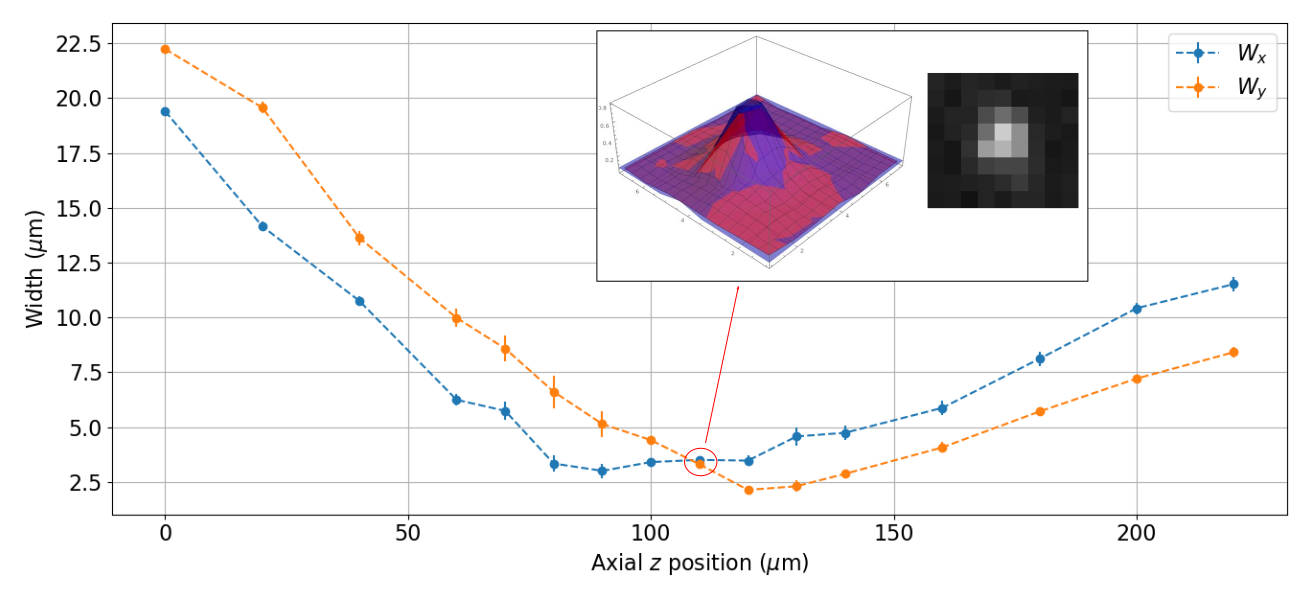
\includegraphics[width=1\textwidth]{cameraprofile}
\caption{Profile of the Gaussian beam}
\label{cameraprofile}
\end{figure}

\subsection{Polarization}
As discussed in the design section, polarization is an important component of the Raman process, thus the polarization capabilities of the system had to be tested. The goal is to achieve vertical, horizontal, left circular, and right circular polarization at the ion position. Polarization can be changed with two plates: a half wave plate after the AOD, and a quarter wave plate right before the objective, see figure \ref{addressingsetup}. In order to characterize the polarization, the three Stokes parameters \cite{stokes} has been measured with a polarimeter from Sc\"after + Kirchhoff series SK010PA. Stokes parameters quantify the type of polarization of an electric field. Linear polarized light (vertical and horizontal) has all Stokes parameters set to 0, apart from the first one. Instead, the third parameter, when the others are zero, contains information about circular polarized light which goes from right to left. By rotating a plate and fitting a sine function to the appropriate Stokes parameter, it is possible to gain insights on the appropriate angle to set in order to obtain the desired polarization.\\
 The first step was to characterize the $\lambda/2$ plate alone, the main result from this characterization is that horizontal polarization can be achieved with an angle of $267.2\pm 0.1 ^{\circ}$, and vertical is achieved with an angle of $312.5\pm0.1^{\circ}$ obtained from fitting a sine on the first Stokes parameter. From the same fit, the semiperiod of the polarization is $45.3\pm 0.6^\circ$.\\
As the mirror can change the polarization, the same characterization has been done after the mirror finding that the polarization is altered unless it is either horizontal or vertical.
However the main result was obtained when the $\lambda/4$ was characterized. With every plate inserted, two measurements were made. In the first one the $\lambda/2$ was set to $267^\circ$ to get horizontal polarization, and the angle of the $\lambda/4$ scanned. This result is presented in figure \ref{pol1}. The third Stokes parameter is fitted with a sine function to get the angles at which the polarization is right and left circular. The right circular polarization is obtained at the maximum of the curve, while the left corresponds to the minimum. Moreover, when the third Stokes parameter is zero, the polarization results linear. The results are shown in table \ref{polarizationstable}.
The second measurement also scanned the angle of the $\lambda/4$ plate, but this time the $\lambda/2$ was set to $312^\circ$ such that the polarization before the $\lambda/4$ plate was vertical. In figure \ref{pol2} the data is displayed. Again, to get the angle for the different polarizations, a sine function was fitted to the third Stokes parameter. The results yielded by the fit are summarized in table \ref{polarizationstable}.

\begin{table}
\centering
\begin{tabular}{c c c}
 \toprule
    {Polarization} & {$\lambda/2$ ($^\circ$)} & {$\lambda/4$ ($^\circ$)} \\ \midrule\midrule
   Horizontal & $267.2\pm 0.1$ & $49.7\pm0.1$  \\
   Vertical   & $312.5\pm0.1$ & $48.1\pm0.1$\\ \midrule
   Right circular & $267.2\pm 0.1$ & $4\pm 0.1$ \\
   Right circular & $312.5\pm0.1$ & $93.1\pm0.1$\\\midrule
  Left circular & $267.2\pm 0.1$ & $95.4\pm0.1$\\
    Left circular & $312.5\pm0.1$  & $3.1\pm0.1$\\ \bottomrule
\end{tabular}
\caption{Angles}
\label{polarizationstable}
\end{table}


\begin{figure}
\centering
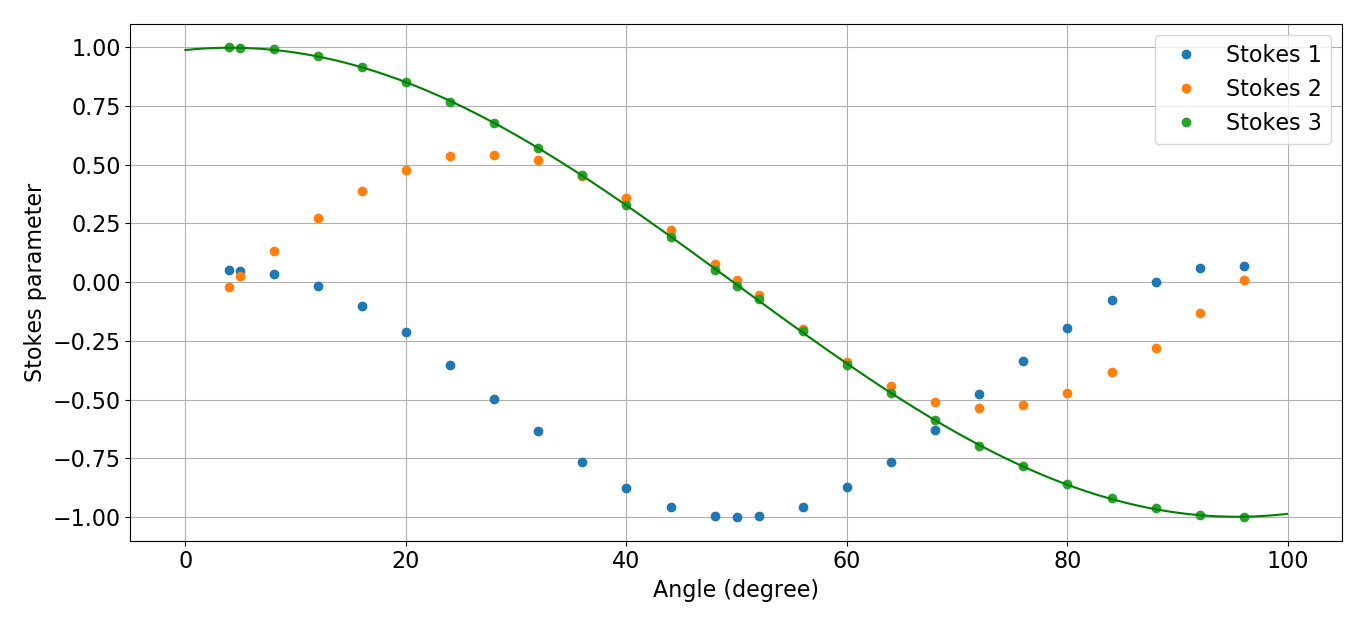
\includegraphics[width = \textwidth]{pol1}
\caption{Polarization after the objective as a function of the $\lambda/4$ angle with $\lambda/2$ set to horizontal ($267^\circ$). Green line is a sine function fit.}
\label{pol1}
\end{figure}

\begin{figure}
\centering
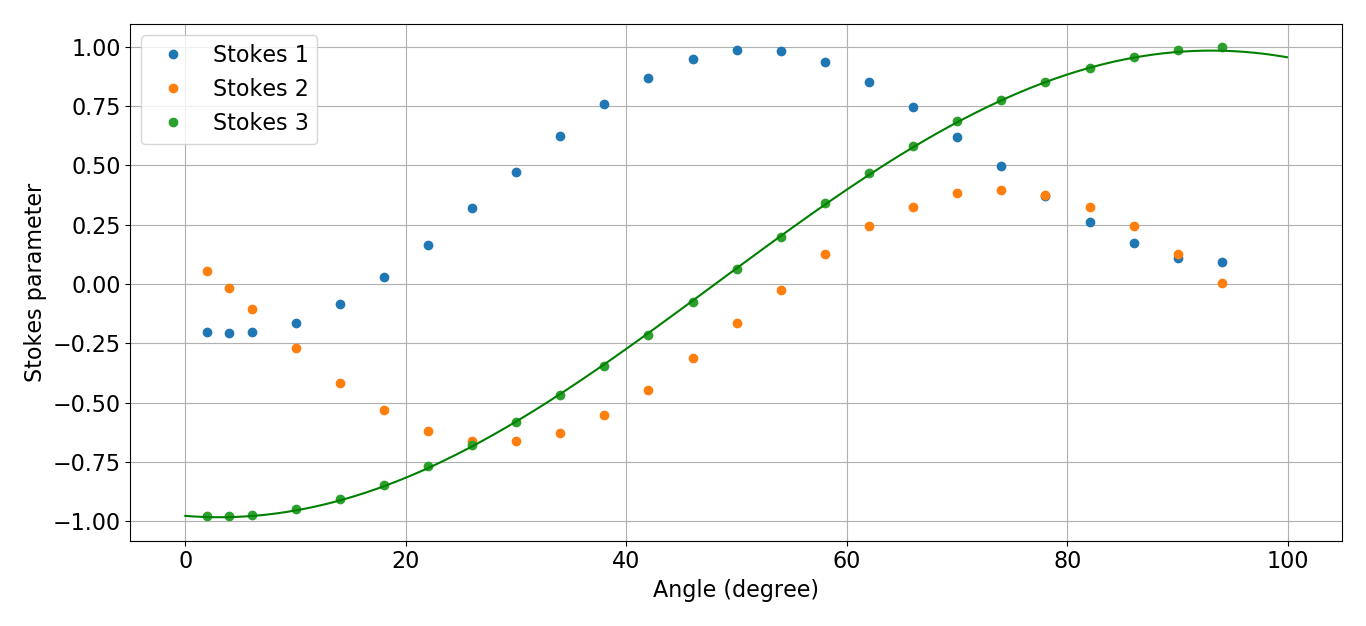
\includegraphics[width = \textwidth]{pol2}
\caption{Polarization after the objective as a function of the $\lambda/4$ angle with $\lambda/2$ set to vertical ($314^\circ$). Green line is a sine function fit.}
\label{pol2}
\end{figure}

\subsection{Stability}
In the future the addressing system will be used for long experiments, it is therefore imperative to know the stability of the system in terms of polarization and beam pointing.
This means knowing over the course of hours or days if the setup needs to be calibrated. Let us start with polarization stability, the polarization was measured with a polarimeter from Sc\"after + Kirchhoff series SK010PA after the objective. The polarization was set to be right circular: $\lambda/2$ set to $267^\circ$, and $\lambda/4$ set to $4^\circ$. We recorded the three Stokes parameters for a total of one hour, this data is plotted in figure \ref{polstability}. To the third parameter, 0.998 has been subtracted during the plot such that it would fit with the others. It can be seen that the polarization is stable over a period of one hour.\\
Beam pointing stability regards the stability of the focus position, which could drift in any direction for any reason. To test the stability, we recorded the position of the focus for a period of one hour with the camera IDS model UI-1490LE-M-GL. The camera was position at the focus with the same setup discussed in section \ref{waistcamera}, and then a video was recorded. The video was later analyzed by tracking the the brightest pixel over time. In figure \ref{beampointing} we can see the horizontal $x$ and vertical $y$ position of such pixel. In the horizontal directions, fluctuations of one single pixel can be noticed, which could be a result of the light hitting between two pixels. In the vertical direction over it looks like the fluctuations are on the order of two pixels, if one consider one pixel a normal fluctuation, then the position might have shifted by one pixel over this period. This means that the focus position is stable with an upperbound of $1.6\,\mu$m/hour.

\begin{figure}[H]
\centering
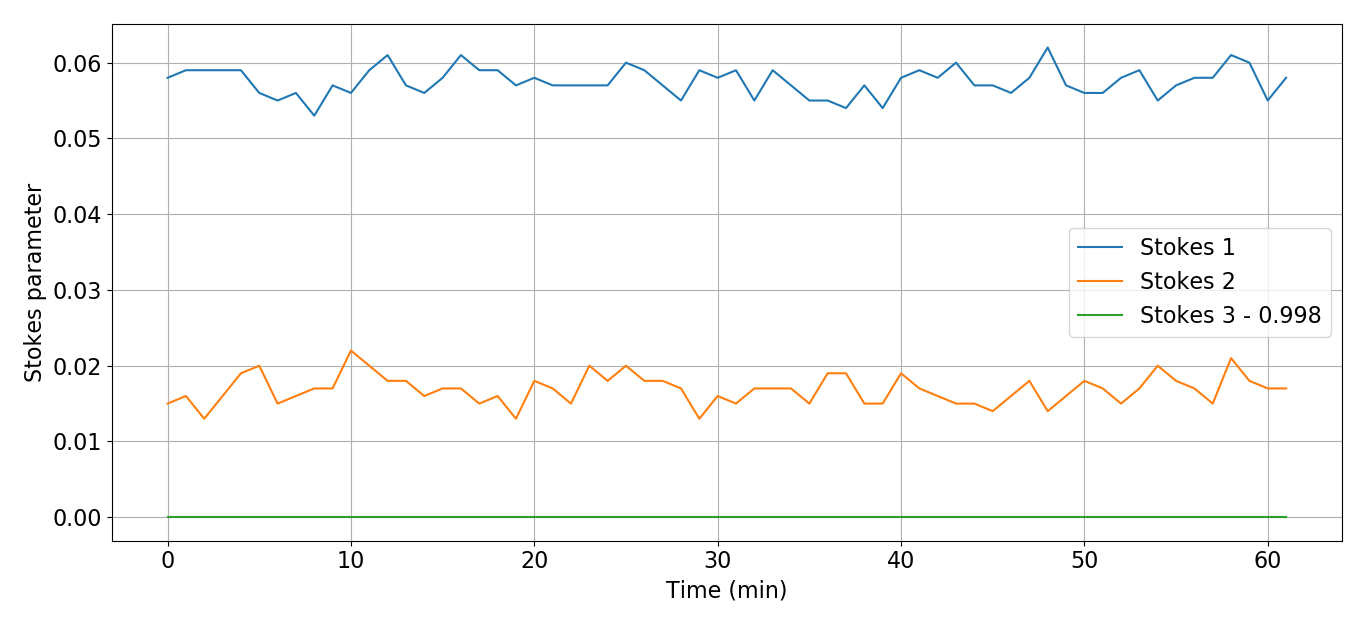
\includegraphics[width = \textwidth]{polstability}
\caption{Right circular polarization stability over a period of one hour.}
\label{polstability}
\end{figure}

\begin{figure}[H]
\centering
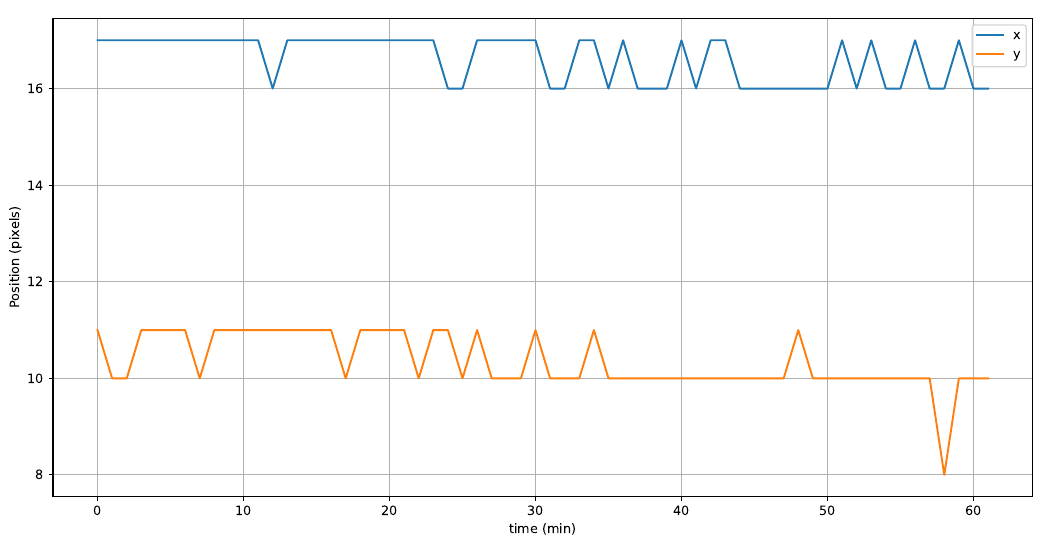
\includegraphics[width = \textwidth]{beampointing}
\caption{Beam pointing stability over a period of one hour.}
\label{beampointing}
\end{figure}


\newpage
\section{Final installed system}
After the tests presented in the previous sections, the setup was installed next to the ion chamber and focused on the ions as described in section \ref{design4}. As there is no more physical access to the focus spot, more advanced quantum optics experiment have to be be carried out in order to measure properties of the system as focus spot and addressing error. The first experiment designed aims exactly at measuring these two quantities: Ramsey fringes were measured on four loaded ions, from which the beam shape can be inferred.
The second experiment that we have done involves three ions and the goal was to generate photons via Raman process from one single ion leaving the state of the other two unaltered, demonstrating therefore the possibility to emit single photons from individual ions in a string.

\subsection{Ramsey interferometry}
Ions can be used as sensitive tools for beam profiling, unfortunately the 393 nm light excites a dipole transition with a short lived excited state. Therefore, a direct excitation followed by a measurement is not fast enough to gain any information. Ideally, the 729nm qubit transition should be used, as here state readout is available and the transition is metastable. This is possible as the 393nm transition shares the ground state with the qubit transition, so the 393nm laser can be detuned such that the AC stark shift caused changes the phase of the qubit producing measurable effects. Measurements of the Stark shift can be done with a Ramsey interference experiment \cite{starkshift}.
The idea of the experiment is to send a resonant $\pi/2$ pulse at 729nm, which bring the qubit state to a superposition $\ket{S}+\ket{D}$, here another in phase resonant $\pi/2$ pulse at 729nm would bring the final state to the excited level $\ket{D}$. However, if between the two 729nm pulses, AC stark shift is induced by a pulse of 393nm light, an additional phase is added to the superposition $\ket{S}+\ket{D}$, and the final state after the second 729nm pulse will depend on the shift induced by the 393nm laser. By calculating the final probability $P_D$ it is possible to infer the power of the 393nm light. Rigorous mathematic can be done with matrices \eqref{laserpulse} here called $U_{729}$ and \eqref{acstarkrotation}, referred to as $U_{393}$. After the three pulse sequence the final state is
\begin{equation}
\begin{split}
\ket{\psi_f} &= U_{729}(\pi,\phi)U_{393}(\delta)U_{729}(\pi,0)\ket{S} \\
&= \frac{1}{2}\left(e^{-i\frac{\delta}{2}t}-e^{-i\phi}\right)\ket{S}-\frac{i}{2}\left(1 + e^{-i\frac{\delta}{2}t} e^{-i\phi}\right)\ket{D}
\end{split}
\end{equation}
where $\delta = \Omega^2/4\Delta$ is the Stark shift, and $\Omega$ is the Rabi frequency of the 393nm light that we want to measure. The final probability is then
\begin{equation}
P_D = \cos^2\left(2\phi + 2\frac{\delta t}{2}\right) = \cos^2\left(2\phi + \frac{\Omega^2 t}{4\Delta}\right).
\end{equation}
As we can see, the final signal depends on the phase of the second 729nm pulse $\phi$ and on the Stark shift induced by the 393nm laser. To get $\Omega^2$ a simple formula inversion can be done $\Omega^2 = \left[\text{arccos}\left(\sqrt{P_D}\right)-2\phi \right]$. The phase $\phi$ can be chosen freely and all constants have been dropped as the data will be normalized.\\
\begin{figure}
\centering
\includegraphics[width=\textwidth]{sequence}
\caption{Experiment sequence}
\label{sequence}
\end{figure}
The experiment sequence is in figure \ref{sequence}, for every sequence, a stage of Doppler Cooling at the beginning is included, and at the end of the pulses PMT readout is performed. The sequence is then repeated $N$ times to estimate the excitation probability for every data point. Between the Raman pulse and the second $\pi/2$ pulse, there is also a dead time which can be adjusted to improve signal to noise ratio.\\
The 393nm pulse has to be off resonance from the transition to avoid spontaneous scattering in the $\text{S}_{1/2}\to \text{P}_{1/2}$ transition. The detuning is therefore chosen such that the ratio of the Stark shift $\delta$ and the spontaneous scattering rate $\Gamma_{eff}$ si at least 100. Using the value from table \ref{transitiontable}
\begin{equation}
\frac{\delta}{\Gamma_{eff}} = \frac{2\Delta}{\Gamma} \implies \Delta \sim 3\,\text{GHz}.
\end{equation}
Once the lasers were all set, four ions were loaded with endcap voltages of 714 V and 700V, and the parameters of the experiment optimized. What has to be found for the experiment is the length of a $\pi/2$ pulse of 729 light and the length $\tau$ of the 393nm pulse. For the first parameter, Rabi flops were measured and the length of the $\pi/2$ pulse is directly estimated to be 4.2 $\mu$s. These flops are showed in figure \ref{rabiflops4}
\begin{figure}[H]
\centering
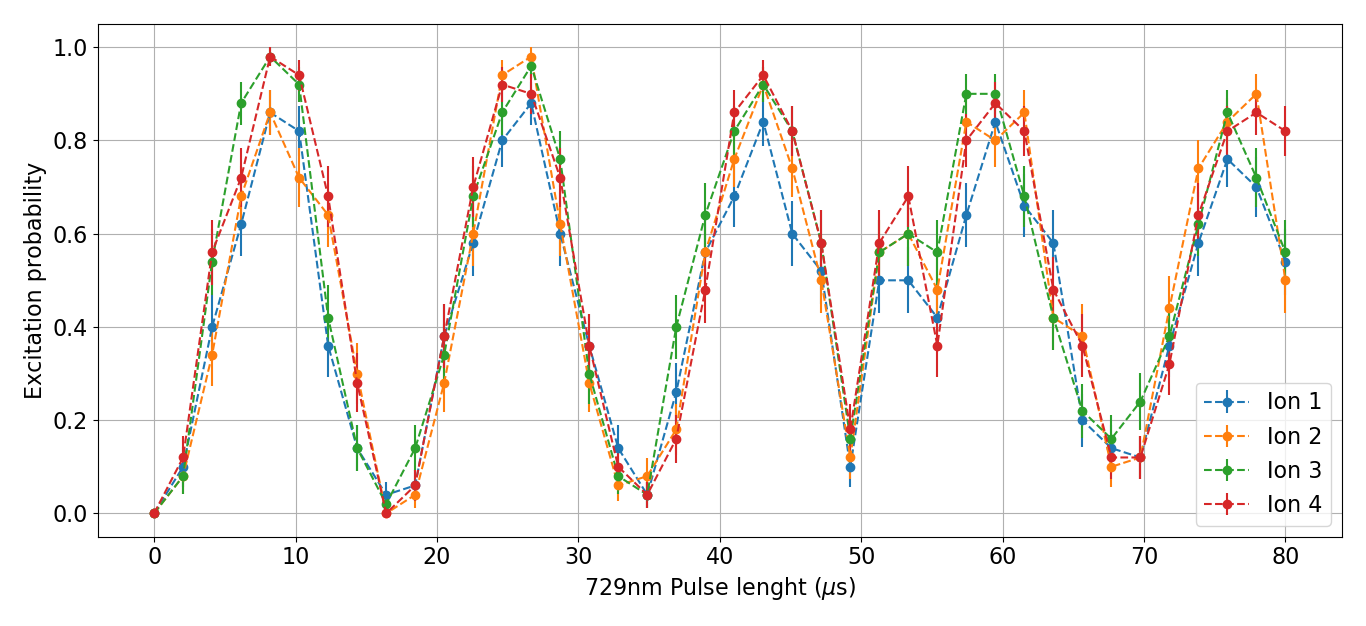
\includegraphics[width=\textwidth]{rabiflops4}
\caption{Rabi flops on 4 ions.}
\label{rabiflops4}
\end{figure}
Errorbars on the excitation probability have been assigned according to the error on estimating the probability of a binomial distribution with $N$ number of repetitions.
\begin{equation}
\sigma = \sqrt{\frac{P_{D}(1-P_{D})}{N}}.
\end{equation}
With this value of $\pi/2$ Ramsey fringes were measured, here the $\phi$ between the two pulses is scanned such that we can decide where to sit for the experiment with the 393nm.
The fringes are in figure \ref{ramseyfringes}, as expected the curve follow a $\cos^2(\phi)$ behaviour. In order to get a better signal, one can decide to sit at the minimum of the curve, i.e. we set for the rest of the experiment $\phi = \pi/2$. The last parameter that has to be decided is the Raman length $\tau$, this value is chosen in a way that the shift caused by the 393nm light does not skip any fringe. This means that if we start from the minimum of figure \ref{ramseyfringes}, the Raman pulse should give an shift that brings the ion at maximum at excitation probability 1, without going further. To get this timing, $\tau$ can be scanned and the appropriate value can be visually chosen, the plot is in figure \ref{ACscan}. We set $\tau$ to be $25\,\mu$s, so we climb only about halfway the fringe. Lastly we set the dead time to be $5\,\mu$s.
\begin{figure}[H]
\centering
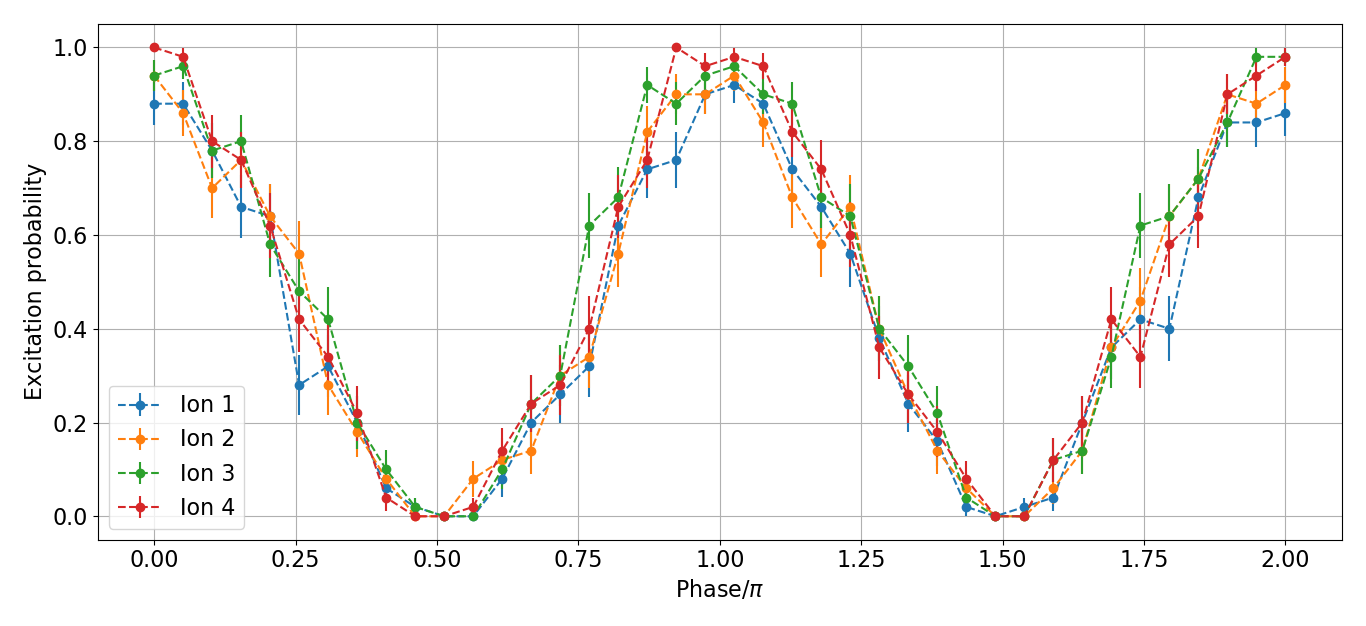
\includegraphics[width=\textwidth]{ramseyfringes}
\caption{Ramsey fringes for 4 ions.}
\label{ramseyfringes}
\end{figure}
To get the profile of the addressing beam, the AOD frequency can be now scanned. During this scan the beam is moved from ion to ion and its shape is probed by the ions. The result
after post analysis can be seen in figure \ref{AODscan}. Here the intensity of the beam has been determined from the probability $P_D$ as discussed, errors are propagated accordingly.
\begin{figure}[H]
\centering
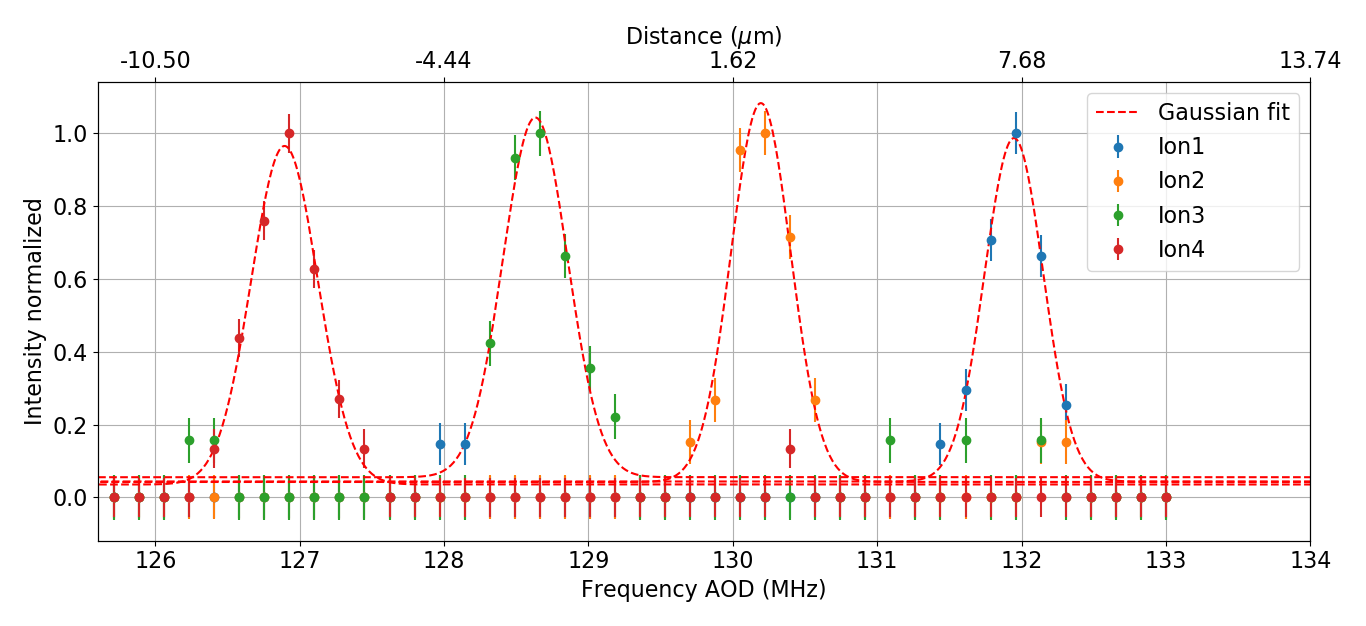
\includegraphics[width=\textwidth]{img/AODScan}
\caption{AOD scanning four ions.}
\label{AODscan}
\end{figure}
To calibrate the micrometer scale, the position in MHz of two peaks have been taken, then from the axial frequency the position of the ions in the trap can be estimated (cfr. section \ref{ionstrings}), by comparing the two values the conversion factor is found.\\
The four peaks have been fitted with a Gaussian function to obtain the waist of the beam when focused on the different ions. The waist yielded by the fits are from right to left are
$\omega_1 = 1.23\pm 0.20\,\mu$m, $\omega_2 = 1.25\pm 0.19\,\mu$m, $ \omega_3 = 1.35\pm 0.22\,\mu$m, $\omega_4 = 1.39\pm 0.20\,\mu$m.\\
The addressing error can also be estimated from the Stark flops in figure \ref{ACscan}. In this measurement, the addressing beam was focused on one ion and the Raman length $\tau$ is scanned. This increases the interaction time of the laser with the ions, and if the interaction is long enough even the tail of a Gaussian can induce some excitation on the ions on the side of the one being addressed. In the scan displayed, the pulse reached 300 $\mu$s and there is no excitation on any ion apart from the one flopping. Others scans went up to 500 $\mu$s, and still no visual excitation is present. While this means that no quantitative number can be determined for the addressing error, an upper bound can still be given. For an excitation to appear right after 500 $\mu$s, the addressing error should be at most $\Omega_2^2/\Omega_3^2< 10^{-3}$ (?)


\begin{figure}[H]
\centering
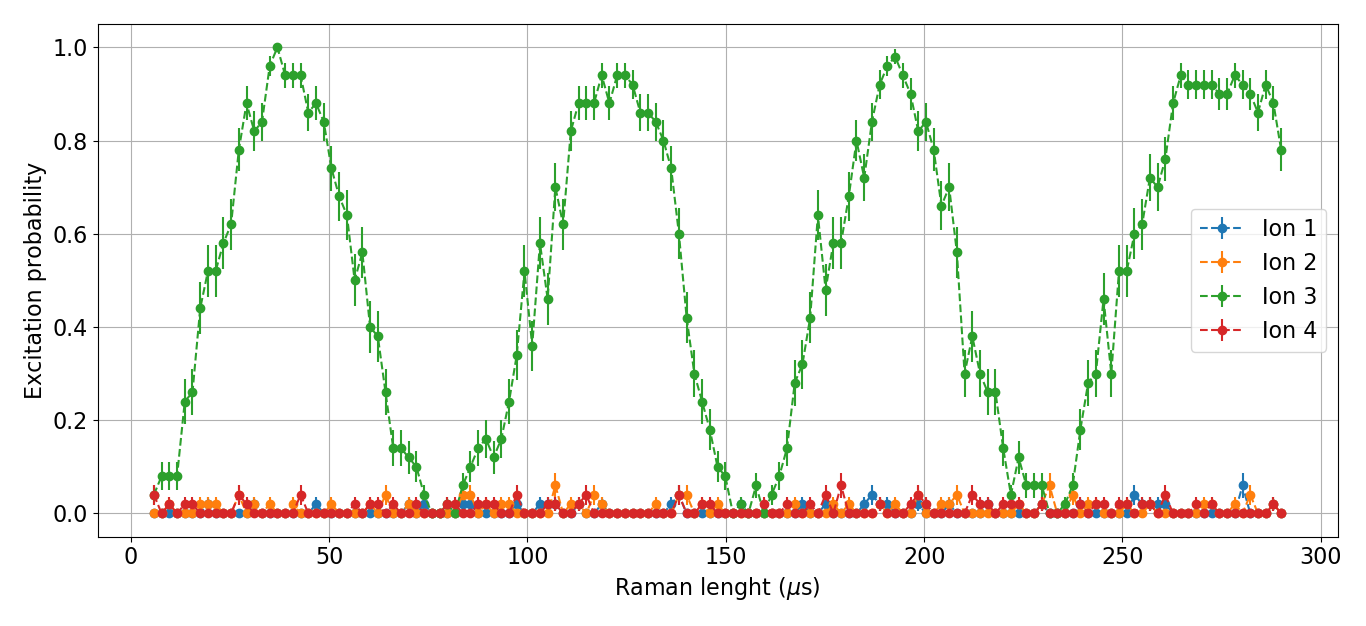
\includegraphics[width=\textwidth]{img/ACscan}
\caption{393nm AC-Stark flops}
\label{ACscan}
\end{figure}

\subsection{Photon production}
\label{exp:photons}
The main goal of having an addressed 393nm setup is to generate single photon from individual ion in a chain. In this experiment we tested this feature by loading a string of 3 ions, and monitoring the photon generation and the ions state as well. A single photon is produced by a pulse of 393nm light focused on the central ion of three via Raman process. In the experiment we scanned the length of this pulse to obtain an integrated wavepacket, i.e. the cumulative probability of detecting a photon as a function of the pulse length. The generated photon is emitted into the cavity, transmitted through a mirror and couple into a fiber that goes to a superconducting nanowire single-photon detector (SNSPD) which clicks if a photon is detected. The detectors have two channels corresponding to two different photon polarizations. Detuning of the Raman laser is essential in this experiment, so one has to take into account the frequency shift induced by the AOD $\sim 127$ MHz. As already briefly mentioned, the shift was compensated with the two AOM's in the 393nm laser setup. The experiment includes an initial stage of Doppler cooling and a final stage of state detection. Furthermore, the locking light 806nm in the cavity was switched off during the photon generation process, in this time the cavity maintained its position with a sample and hold. The measurement is repeated $N$ times to get the average photon probability and the excitation probability. These two quantities are plotted in figure \ref{probphoton} and \ref{probion}.
\begin{figure}[H]
\centering
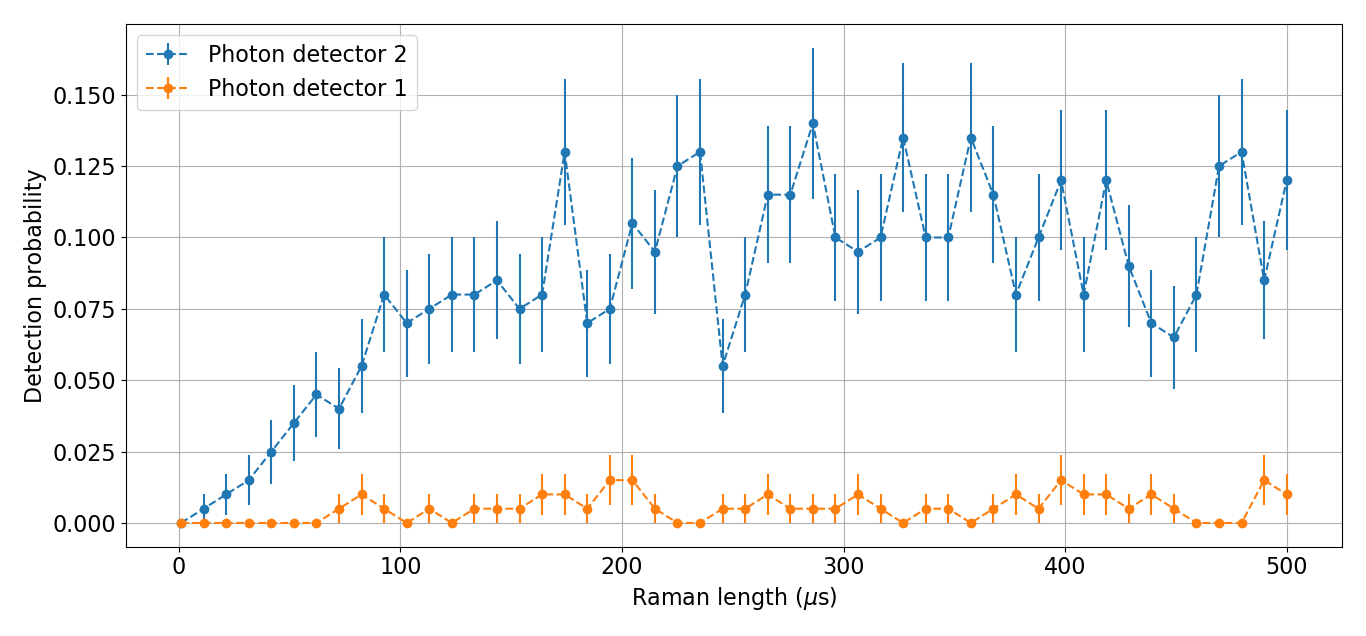
\includegraphics[width=\textwidth]{img/photonefficency_witherror}
\caption{Generated photon efficency}
\label{probphoton}
\end{figure}
\begin{figure}[H]
\centering
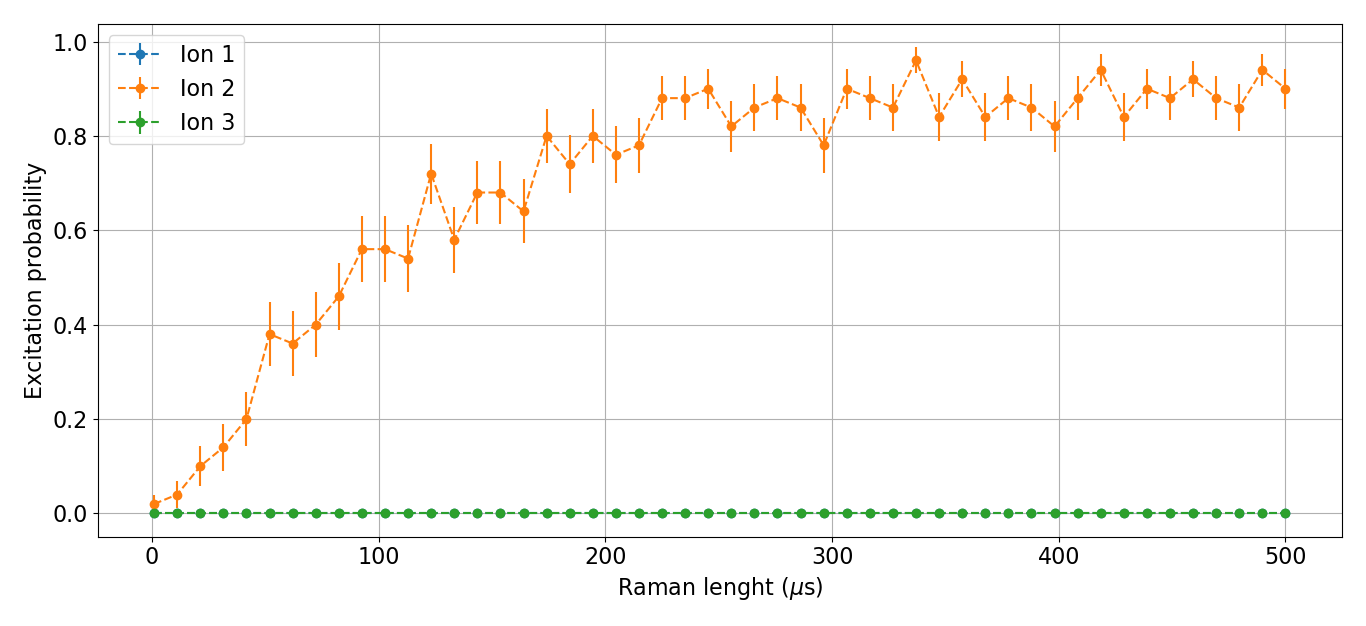
\includegraphics[width=\textwidth]{img/ramanlength_witherrors}
\caption{Excitation of ion while emitting photon}
\label{probion}
\end{figure}
Errorbars on the excitation probability are calculated as the previous section, while for the photon probability the error is given by Poissonian statistics []
\begin{equation}
\sigma_{ph} = \frac{\sqrt{N_{click}}}{N},
\end{equation}
where $N_{click}$ is the number of times a photon has been detected with respect to the total $N$ repetitions.
As we can see, only the addressed ion gets excited as emits a photon. The probability of getting photon is relatively low $<15 \%$, as no optimization were performed to increase it.

\section{Final properties summary}
?
